\documentclass[10pt,a4paper]{report}
\usepackage[latin1]{inputenc}
\usepackage{amsmath}
\usepackage{amsfonts}
\usepackage{amssymb}
\usepackage{graphicx}
\author{Roberto Capobianco and Jacopo Serafin}
\title{Report: Best Face Pose Detection}
\begin{document}
\maketitle
\section*{Introduction and Problem Statement}
Face detection is a particular subset of object-class detection. Differently from object-class detection, where the goal is to find the locations and sizes of all objects in an image that belong to a given class, face-detection algorithms focus on the detection of human faces.

Face detection is a fundamental building block of many applications, like:
\begin{description}
  \item[Facial Recognition] A computer application for automatically identifying a person from a digital image or a video frame. One possible way to do this is by comparing facial features between the image and a facial database.
  \item[Photography] In recent digital cameras a basic features like the auto focus uses face detection to find regions in the image to focus.
  \item[Social Media] Suggest to tag a friend in a photo is a basic peculiarity of almost all social network.
\end{description}
The most famous and commonly used approach to face detection is the Viola-Jones algorithm \cite{viola2004robust}. It is based on a set of features which involve the sums of image pixels within rectangular areas (integral images). Specifically, they are a more complex version of Haar basis functions, which have been used previously in image-based object detection \cite{papageorgiou}, since they rely on more than one rectangular area. \figurename~\ref{fig:haar_features} shows the types of features used in the framework presented by Viola and Jones. 
\begin{figure}
\centering
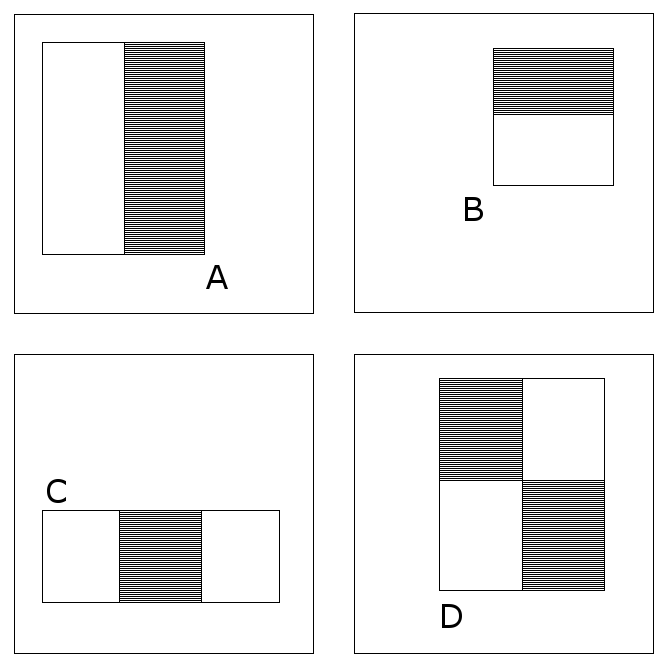
\includegraphics[width=0.5\textwidth]{./haar_features.png}
\caption{Haar-like features used in the Viola-Jones algorithm}
\label{fig:haar_features}
\end{figure}
By using integral images, rectangular features can be evaluated in constant time, obtaining in this way a valuable speed-up over their more complex relatives, like steerable filters \cite{steerable}.
In many applications, however, being able to recognize frontal poses (or "best poses") in a video sequence or in a photo is a fundamental part since it improves drastically the results. For example, if we want to recognize a user, by comparing his face with a database of previously acquired faces, we need to have them in similar poses.
Our aim is to construct a system which is able to better detect frontal poses of a single person in a video source. This is based on geometrical constraints on facial features.

\section*{Methodology}
Our method is based on two fundamental steps: the first one is the face detection, along with the eyes and the mouth, in a video sequence; the second step is the worst pose rejection based on a series of geometric constraints related to the previously extracted facial features.
\subsection*{Feature Detection}
As already stated, the first phase of the algorithm is to find, in real time, the face, eyes and mouth inside each frame of a video source stream. This activity is performed by exploiting the Viola-Jones method implementation of the OpenCV library\footnote{http://opencv.org/}. More in detail we apply the following processing steps, in a hierarchical manner:
\begin{enumerate}
\item Video stream opening and frame analysis;
\item Face detection on the whole image, by means of the haar-like cascades both for frontal and profile faces: the face which is selected among the alternatives is the most visible one or, more formally, the face with the biggest area;
\item Eyes detection on the portion of the image belonging to the detected face: constraints on the distance of the two eyes are added in order to improve the detection results, removing many false positives;
\item Mouth detection on the sub-portion of image belonging to the detected face and under the eyes;
\end{enumerate}
Visual evidence of the obtained results is available from \figurename~\ref{fig:facedetect}, where both a frontal and a profile face are detected.
\begin{figure}
\centering
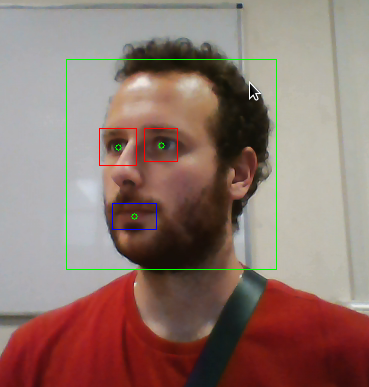
\includegraphics[width=0.4\textwidth]{./jacopo_facedetect.png}
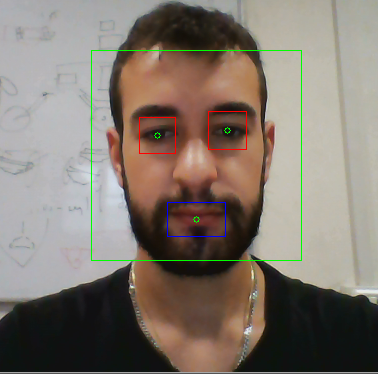
\includegraphics[width=0.424\textwidth]{./rob_facedetect.png}
\caption{Face detection results. A green rectangle contains the detected face, while the red and the blue rectangles contains, respectively, the eyes and the mouth resulting from the detection phase.}
\label{fig:facedetect}
\end{figure}
\subsection*{Best Pose Selection}
The second processing phase consists in the application of some heuristics for the selection of the best pose, in the video, for the detected face. Namely, a pose is considered to be good when the face is frontal with respect to the camera. In order to obtain good poses, we evaluate some metrics between the key points of the face previously detected (eyes and mouth central points). In detail, we consider
\begin{enumerate}
\item Eyes vertical distance: since we do not apply rotation correction, we only accept poses in which the face is not rotated and, therefore, the vertical distance between the eyes is below a threshold corresponding to 7\% of face height;
\item Angles between eyes and mouth: by computing the segment between the two eyes and those between the eyes and the mouth we evaluate the eye angles. In particular, we compare the two angles in such a way to evaluate their difference with respect to a reference of 67.5°. This value has been found empirically, by measuring the eye angles on a set of different frontal poses in several video streams.
\end{enumerate}
\section*{Results}
Good results \figurename~\ref{fig:best_pose}
\begin{figure}
\centering
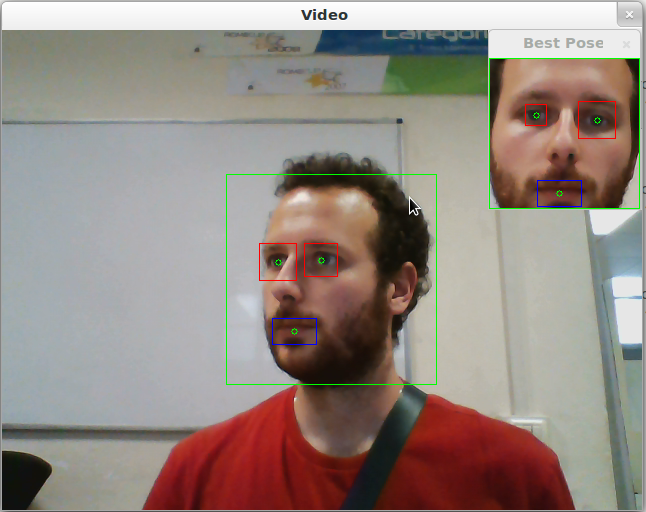
\includegraphics[width=0.9\textwidth]{./best_face_jacopo.png}
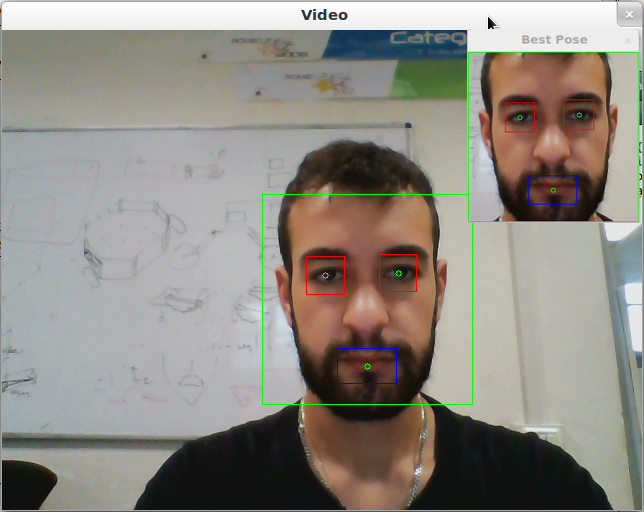
\includegraphics[width=0.9\textwidth]{./best_face_rob.png}
\caption{Results of the best face pose detection. The top image shows a profile face and the best pose, which is not updated to the new frame. The bottom image, instead, shows that when the pose is good (frontal) the best pose window is updated with the new frame.}
\label{fig:best_pose}
\end{figure}
\section*{Conclusions}
In this project we applied the Viola-Jones algorithm in order to detect faces. In detail, we detected in a hierarchical manner also eyes and mouth and we used this key points in the face to determine some metrics. These metrics have been used as heuristics for the selection of the best poses in several video streams, obtaining good performances.

\begin{thebibliography}{9}

\bibitem{viola2004robust}
Viola, Paul, and Michael J. Jones. \emph{``Robust real-time face detection."} International journal of computer vision 57.2 (2004): 137-154.

\bibitem{papageorgiou}
Papageorgiou, Constantine P., Michael Oren, and Tomaso Poggio. \emph{``A general framework for object detection."} Computer vision, 1998. sixth international conference on. IEEE, 1998.

\bibitem{steerable}
Freeman, William T., and Edward H. Adelson. \emph{``The design and use of steerable filters."} IEEE Transactions on Pattern analysis and machine intelligence 13.9 (1991): 891-906.

\end{thebibliography}
\end{document}